\documentclass{eptcs}

% Define to fix sigplanconf.
% \doi{}

\setlength{\paperheight}{11in}
\setlength{\paperwidth}{8.5in}
\usepackage[
  pass,% keep layout unchanged 
  % showframe,% show the layout
]{geometry}

% LNCS: creates bib on new page with centered title
\usepackage[square,comma,numbers,sort&compress]{natbib}
%\usepackage[hyphens]{url}
%\usepackage[breaklinks,colorlinks]{hyperref}
\usepackage[usenames,dvipsnames]{xcolor}
\hypersetup{citecolor=blue,linkcolor=blue}
\usepackage{amsthm}
\usepackage{amsmath,amsopn,amssymb}
\usepackage{subfig}
\usepackage{endnotes,microtype,xspace,graphicx,fancyvrb,multirow}
\usepackage{booktabs}
\usepackage{array,underscore,relsize}
\usepackage[T1]{fontenc}
% \usepackage{times}
\usepackage{fancyhdr,lastpage}
\usepackage{enumitem}
% Makes sigplanconf throw warning.
% \usepackage[labelfont=bf,font=small,skip=5pt]{caption}

% aliascnt: counter stuff that works with theorem environments.
\usepackage{aliascnt}
\usepackage{listings}

% algorithm2e: algorithms
\usepackage[linesnumbered]{algorithm2e}

% semantic: inference rules
\usepackage{semantic}

% stmaryrd: more math fonts (namely mathbb)
\usepackage{stmaryrd}

% floatrow: putting two figures side by side
\usepackage{floatrow}

\usepackage{mathtools}
\usepackage{tikz}
\usetikzlibrary{positioning}
\usetikzlibrary{automata}
\usetikzlibrary{shapes}

\pagestyle{fancy}
\fancyhf{}
\renewcommand{\headrulewidth}{0pt}
\cfoot{\thepage}

\newcommand{\sys}{\mbox{\textsc{Shara}}\xspace}

% cmds: typesetting commands
\renewcommand{\ttdefault}{pxtt}

\newcommand{\URL}{\url}
\newcommand{\cc}[1]{\mbox{\smaller[0.5]\texttt{#1}}}

%\clubpenalty=10000
%\widowpenalty=10000

%\linespread{1.2}

\fvset{fontsize=\scriptsize,xleftmargin=8pt,numbers=left,numbersep=5pt}


\makeatletter
\def\PY@reset{\let\PY@it=\relax \let\PY@bf=\relax%
    \let\PY@ul=\relax \let\PY@tc=\relax%
    \let\PY@bc=\relax \let\PY@ff=\relax}
\def\PY@tok#1{\csname PY@tok@#1\endcsname}
\def\PY@toks#1+{\ifx\relax#1\empty\else%
    \PY@tok{#1}\expandafter\PY@toks\fi}
\def\PY@do#1{\PY@bc{\PY@tc{\PY@ul{%
    \PY@it{\PY@bf{\PY@ff{#1}}}}}}}
\def\PY#1#2{\PY@reset\PY@toks#1+\relax+\PY@do{#2}}

\expandafter\def\csname PY@tok@gd\endcsname{\def\PY@tc##1{\textcolor[rgb]{0.63,0.00,0.00}{##1}}}
\expandafter\def\csname PY@tok@gu\endcsname{\let\PY@bf=\textbf\def\PY@tc##1{\textcolor[rgb]{0.50,0.00,0.50}{##1}}}
\expandafter\def\csname PY@tok@gt\endcsname{\def\PY@tc##1{\textcolor[rgb]{0.00,0.27,0.87}{##1}}}
\expandafter\def\csname PY@tok@gs\endcsname{\let\PY@bf=\textbf}
\expandafter\def\csname PY@tok@gr\endcsname{\def\PY@tc##1{\textcolor[rgb]{1.00,0.00,0.00}{##1}}}
\expandafter\def\csname PY@tok@cm\endcsname{\let\PY@it=\textit\def\PY@tc##1{\textcolor[rgb]{0.25,0.50,0.50}{##1}}}
\expandafter\def\csname PY@tok@vg\endcsname{\def\PY@tc##1{\textcolor[rgb]{0.10,0.09,0.49}{##1}}}
\expandafter\def\csname PY@tok@vi\endcsname{\def\PY@tc##1{\textcolor[rgb]{0.10,0.09,0.49}{##1}}}
\expandafter\def\csname PY@tok@mh\endcsname{\def\PY@tc##1{\textcolor[rgb]{0.40,0.40,0.40}{##1}}}
\expandafter\def\csname PY@tok@cs\endcsname{\let\PY@it=\textit\def\PY@tc##1{\textcolor[rgb]{0.25,0.50,0.50}{##1}}}
\expandafter\def\csname PY@tok@ge\endcsname{\let\PY@it=\textit}
\expandafter\def\csname PY@tok@vc\endcsname{\def\PY@tc##1{\textcolor[rgb]{0.10,0.09,0.49}{##1}}}
\expandafter\def\csname PY@tok@il\endcsname{\def\PY@tc##1{\textcolor[rgb]{0.40,0.40,0.40}{##1}}}
\expandafter\def\csname PY@tok@go\endcsname{\def\PY@tc##1{\textcolor[rgb]{0.53,0.53,0.53}{##1}}}
\expandafter\def\csname PY@tok@cp\endcsname{\def\PY@tc##1{\textcolor[rgb]{0.74,0.48,0.00}{##1}}}
\expandafter\def\csname PY@tok@gi\endcsname{\def\PY@tc##1{\textcolor[rgb]{0.00,0.63,0.00}{##1}}}
\expandafter\def\csname PY@tok@gh\endcsname{\let\PY@bf=\textbf\def\PY@tc##1{\textcolor[rgb]{0.00,0.00,0.50}{##1}}}
\expandafter\def\csname PY@tok@ni\endcsname{\let\PY@bf=\textbf\def\PY@tc##1{\textcolor[rgb]{0.60,0.60,0.60}{##1}}}
\expandafter\def\csname PY@tok@nl\endcsname{\def\PY@tc##1{\textcolor[rgb]{0.63,0.63,0.00}{##1}}}
\expandafter\def\csname PY@tok@nn\endcsname{\let\PY@bf=\textbf\def\PY@tc##1{\textcolor[rgb]{0.00,0.00,1.00}{##1}}}
\expandafter\def\csname PY@tok@no\endcsname{\def\PY@tc##1{\textcolor[rgb]{0.53,0.00,0.00}{##1}}}
\expandafter\def\csname PY@tok@na\endcsname{\def\PY@tc##1{\textcolor[rgb]{0.49,0.56,0.16}{##1}}}
\expandafter\def\csname PY@tok@nb\endcsname{\def\PY@tc##1{\textcolor[rgb]{0.00,0.50,0.00}{##1}}}
\expandafter\def\csname PY@tok@nc\endcsname{\let\PY@bf=\textbf\def\PY@tc##1{\textcolor[rgb]{0.00,0.00,1.00}{##1}}}
\expandafter\def\csname PY@tok@nd\endcsname{\def\PY@tc##1{\textcolor[rgb]{0.67,0.13,1.00}{##1}}}
\expandafter\def\csname PY@tok@ne\endcsname{\let\PY@bf=\textbf\def\PY@tc##1{\textcolor[rgb]{0.82,0.25,0.23}{##1}}}
\expandafter\def\csname PY@tok@nf\endcsname{\def\PY@tc##1{\textcolor[rgb]{0.00,0.00,1.00}{##1}}}
\expandafter\def\csname PY@tok@si\endcsname{\let\PY@bf=\textbf\def\PY@tc##1{\textcolor[rgb]{0.73,0.40,0.53}{##1}}}
\expandafter\def\csname PY@tok@s2\endcsname{\def\PY@tc##1{\textcolor[rgb]{0.73,0.13,0.13}{##1}}}
\expandafter\def\csname PY@tok@nt\endcsname{\let\PY@bf=\textbf\def\PY@tc##1{\textcolor[rgb]{0.00,0.50,0.00}{##1}}}
\expandafter\def\csname PY@tok@nv\endcsname{\def\PY@tc##1{\textcolor[rgb]{0.10,0.09,0.49}{##1}}}
\expandafter\def\csname PY@tok@s1\endcsname{\def\PY@tc##1{\textcolor[rgb]{0.73,0.13,0.13}{##1}}}
\expandafter\def\csname PY@tok@ch\endcsname{\let\PY@it=\textit\def\PY@tc##1{\textcolor[rgb]{0.25,0.50,0.50}{##1}}}
\expandafter\def\csname PY@tok@m\endcsname{\def\PY@tc##1{\textcolor[rgb]{0.40,0.40,0.40}{##1}}}
\expandafter\def\csname PY@tok@gp\endcsname{\let\PY@bf=\textbf\def\PY@tc##1{\textcolor[rgb]{0.00,0.00,0.50}{##1}}}
\expandafter\def\csname PY@tok@sh\endcsname{\def\PY@tc##1{\textcolor[rgb]{0.73,0.13,0.13}{##1}}}
\expandafter\def\csname PY@tok@ow\endcsname{\let\PY@bf=\textbf\def\PY@tc##1{\textcolor[rgb]{0.67,0.13,1.00}{##1}}}
\expandafter\def\csname PY@tok@sx\endcsname{\def\PY@tc##1{\textcolor[rgb]{0.00,0.50,0.00}{##1}}}
\expandafter\def\csname PY@tok@bp\endcsname{\def\PY@tc##1{\textcolor[rgb]{0.00,0.50,0.00}{##1}}}
\expandafter\def\csname PY@tok@c1\endcsname{\let\PY@it=\textit\def\PY@tc##1{\textcolor[rgb]{0.25,0.50,0.50}{##1}}}
\expandafter\def\csname PY@tok@o\endcsname{\def\PY@tc##1{\textcolor[rgb]{0.40,0.40,0.40}{##1}}}
\expandafter\def\csname PY@tok@kc\endcsname{\let\PY@bf=\textbf\def\PY@tc##1{\textcolor[rgb]{0.00,0.50,0.00}{##1}}}
\expandafter\def\csname PY@tok@c\endcsname{\let\PY@it=\textit\def\PY@tc##1{\textcolor[rgb]{0.25,0.50,0.50}{##1}}}
\expandafter\def\csname PY@tok@mf\endcsname{\def\PY@tc##1{\textcolor[rgb]{0.40,0.40,0.40}{##1}}}
\expandafter\def\csname PY@tok@err\endcsname{\def\PY@bc##1{\setlength{\fboxsep}{0pt}\fcolorbox[rgb]{1.00,0.00,0.00}{1,1,1}{\strut ##1}}}
\expandafter\def\csname PY@tok@mb\endcsname{\def\PY@tc##1{\textcolor[rgb]{0.40,0.40,0.40}{##1}}}
\expandafter\def\csname PY@tok@ss\endcsname{\def\PY@tc##1{\textcolor[rgb]{0.10,0.09,0.49}{##1}}}
\expandafter\def\csname PY@tok@sr\endcsname{\def\PY@tc##1{\textcolor[rgb]{0.73,0.40,0.53}{##1}}}
\expandafter\def\csname PY@tok@mo\endcsname{\def\PY@tc##1{\textcolor[rgb]{0.40,0.40,0.40}{##1}}}
\expandafter\def\csname PY@tok@kd\endcsname{\let\PY@bf=\textbf\def\PY@tc##1{\textcolor[rgb]{0.00,0.50,0.00}{##1}}}
\expandafter\def\csname PY@tok@mi\endcsname{\def\PY@tc##1{\textcolor[rgb]{0.40,0.40,0.40}{##1}}}
\expandafter\def\csname PY@tok@kn\endcsname{\let\PY@bf=\textbf\def\PY@tc##1{\textcolor[rgb]{0.00,0.50,0.00}{##1}}}
\expandafter\def\csname PY@tok@cpf\endcsname{\let\PY@it=\textit\def\PY@tc##1{\textcolor[rgb]{0.25,0.50,0.50}{##1}}}
\expandafter\def\csname PY@tok@kr\endcsname{\let\PY@bf=\textbf\def\PY@tc##1{\textcolor[rgb]{0.00,0.50,0.00}{##1}}}
\expandafter\def\csname PY@tok@s\endcsname{\def\PY@tc##1{\textcolor[rgb]{0.73,0.13,0.13}{##1}}}
\expandafter\def\csname PY@tok@kp\endcsname{\def\PY@tc##1{\textcolor[rgb]{0.00,0.50,0.00}{##1}}}
\expandafter\def\csname PY@tok@w\endcsname{\def\PY@tc##1{\textcolor[rgb]{0.73,0.73,0.73}{##1}}}
\expandafter\def\csname PY@tok@kt\endcsname{\def\PY@tc##1{\textcolor[rgb]{0.69,0.00,0.25}{##1}}}
\expandafter\def\csname PY@tok@sc\endcsname{\def\PY@tc##1{\textcolor[rgb]{0.73,0.13,0.13}{##1}}}
\expandafter\def\csname PY@tok@sb\endcsname{\def\PY@tc##1{\textcolor[rgb]{0.73,0.13,0.13}{##1}}}
\expandafter\def\csname PY@tok@k\endcsname{\let\PY@bf=\textbf\def\PY@tc##1{\textcolor[rgb]{0.00,0.50,0.00}{##1}}}
\expandafter\def\csname PY@tok@se\endcsname{\let\PY@bf=\textbf\def\PY@tc##1{\textcolor[rgb]{0.73,0.40,0.13}{##1}}}
\expandafter\def\csname PY@tok@sd\endcsname{\let\PY@it=\textit\def\PY@tc##1{\textcolor[rgb]{0.73,0.13,0.13}{##1}}}

\def\PYZbs{\char`\\}
\def\PYZus{\char`\_}
\def\PYZob{\char`\{}
\def\PYZcb{\char`\}}
\def\PYZca{\char`\^}
\def\PYZam{\char`\&}
\def\PYZlt{\char`\<}
\def\PYZgt{\char`\>}
\def\PYZsh{\char`\#}
\def\PYZpc{\char`\%}
\def\PYZdl{\char`\$}
\def\PYZhy{\char`\-}
\def\PYZsq{\char`\'}
\def\PYZdq{\char`\"}
\def\PYZti{\char`\~}
% for compatibility with earlier versions
\def\PYZat{@}
\def\PYZlb{[}
\def\PYZrb{]}
\makeatother


\newcommand{\figrule}{\hrule width \hsize height .33pt}
\newcommand{\coderule}{\vspace{-0.4em}\figrule}

\setlength{\abovedisplayskip}{0pt}
\setlength{\abovedisplayshortskip}{0pt}
\setlength{\belowdisplayskip}{0pt}
\setlength{\belowdisplayshortskip}{0pt}
\setlength{\jot}{0pt}

\def\Snospace~{\S{}}
\renewcommand*\sectionautorefname{\Snospace}
\def\sectionautorefname{\Snospace}
\def\subsectionautorefname{\Snospace}
\def\subsubsectionautorefname{\Snospace}
\def\chapterautorefname{\Snospace}
\def\equationautorefname{Eqn.}

%\renewcommand{\figurename}{Fig.}
%\def\figureautorefname{\figurename}
\newcommand{\subfigureautorefname}{\figureautorefname}

%\numberwithin{equation}{section}
\newcommand{\yes}{Y}
\newcommand{\no}{}

% sema
\newcommand{\shl}{\ \cc{<}\cc{<}\ }
\newcommand{\shr}{\ \cc{>}\cc{>}\ }

\if 0
\renewcommand{\topfraction}{0.9}
\renewcommand{\dbltopfraction}{0.9}
\renewcommand{\bottomfraction}{0.8}
\renewcommand{\textfraction}{0.05}
\renewcommand{\floatpagefraction}{0.9}
\renewcommand{\dblfloatpagefraction}{0.9}
\setcounter{topnumber}{10}
\setcounter{bottomnumber}{10}
\setcounter{totalnumber}{10}
\setcounter{dbltopnumber}{10}
\fi

\newif\ifdraft\drafttrue
\newif\ifnotes\notestrue
\ifdraft\else\notesfalse\fi

% per-author notes:
% ref. http://en.wikibooks.org/wiki/LaTeX/Colors
\newcommand{\BH}[1]{\textcolor{Green}{BH: #1}}
\newcommand{\CV}[1]{\textcolor{Orange}{BH: #1}}
\newcommand{\QZ}[1]{\textcolor{Red}{QZ: #1}}
\newcommand{\DAH}[1]{\textcolor{Blue}{DAH: #1}}

% \newcommand{\TODO}[1]{\textcolor{red}{TODO: #1}}

%% Ensure ligatures (e.g., ``fine official flag'') can be copy/pasted from PDF.
\input{glyphtounicode}
\pdfgentounicode=1

\newcolumntype{R}[1]{>{\raggedleft\let\newline\\\arraybackslash\hspace{0pt}}p{#1}}

% include macros
\newcommand{\includepdf}[1]{
  \includegraphics[width=\columnwidth]{#1}
}

\newcommand{\includeplot}[1]{
  \resizebox{\columnwidth}{!}{\input{#1}}
}

% list
\newcommand{\squishlist}{
\begin{itemize}[noitemsep,nolistsep]
  \setlength{\itemsep}{-0pt}
}
\newcommand{\squishend}{
  \end{itemize}
}

%% NOTE.
%%  to use circled number in caption, use
%%   (e.g., \protect\C{1})
%%
\usepackage{tikz}
\newcommand*\C[1]{%
\begin{tikzpicture}[baseline=(C.base)]
\node[draw,circle,inner sep=0.2pt](C) {#1};
\end{tikzpicture}}

\newcommand*\BC[1]{%
\begin{tikzpicture}[baseline=(C.base)]
\node[draw,circle,fill=black,inner sep=0.2pt](C) {\textcolor{white}{#1}};
\end{tikzpicture}}

\newcommand{\PP}[1]{
\vspace{2px}
\noindent{\bf #1}
}


% std: standard math commands and environments.
% Standard math shorthand.
\newcommand{\add}[2]{#1 \union \{ #2 \}}

\newcommand{\assign}{\mathbin{:=}}

\newcommand{\auflia}{\textsc{Auflia}\xspace}

\newcommand{\bigland}{\bigwedge}

\newcommand{\biglor}{\bigvee}

\newcommand{\bigunion}{\bigcup}

\newcommand{\bools}{\mathbb{B}}

\newcommand{\bv}{\textsc{Bv}\xspace}

\newcommand{\code}{\mathtt}

\newcommand{\compose}{\circ}

\newcommand{\concat}{\cdot}

\newcommand{\cons}{\mathbin{::}}

\newcommand{\disjunion}{\dot{\cup}}

\newcommand{\domain}{\mathsf{Dom}}

\newcommand{\elts}[1]{\{ #1 \}}

\newcommand{\entails}{\models}

\newcommand{\euf}{\textsc{Euf}\xspace}

\newcommand{\false}{\mathsf{False}}

\newcommand{\intersection}{\cap}

\newcommand{\ints}{\mathbb{Z}}

\newcommand{\lia}{\textsc{Lia}\xspace}

\newcommand{\nats}{\mathbb{N}}

\newcommand{\none}{\mathsf{None}}

\newcommand{\partto}{\hookrightarrow}

\newcommand{\pset}{\mathcal{P}}

\newcommand{\range}{\mathsf{Rng}}

\newcommand{\remove}[2]{#1 \setminus \{ #2 \}}

\newcommand{\replace}[3]{#1 [ #3 / #2 ]}

\newcommand{\restrict}[2]{#1|_{#2}}

\newcommand{\sats}{\vdash}

\newcommand{\setformer}[2]{\{ #1\ |\ #2 \}}

\newcommand{\some}{\mathsf{Some}}

\newcommand{\subs}[2]{#1 [ #2 ]}

\newcommand{\tc}[1]{#1^{*}}

\newcommand{\true}{\mathsf{True}}

\newcommand{\undef}{\uparrow}

\newcommand{\union}{\cup}

\newcommand{\upd}[3]{#1[#2 \mapsto #3]}

% Theorem environments
\newtheorem{cor}{\bf{Corollary}}

\newtheorem{defn}{\bf{Definition}}

\newtheorem{ex}{\bf{Example}}

\newtheorem{lem}{\bf{Lemma}}

\newtheorem{thm}{\bf{Theorem}}

% Register classes of stuff to refer to with autoref.
\renewcommand{\algorithmautorefname}{Alg.}

\newcommand{\appautorefname}{App.}

\newcommand{\corautorefname}{Cor.}

\newcommand{\defnautorefname}{Defn.}

\newcommand{\exautorefname}{Ex.}

\newcommand{\figautorefname}{Fig.}

\newcommand{\lemautorefname}{Lemma}

\newcommand{\lineautorefname}{Line}

\newcommand{\thmautorefname}{Thm.}

%%% Local Variables: 
%%% mode: latex
%%% TeX-master: "p"
%%% End: 


% shorthand: paper-specific shorthand commands.
% shorthand: paper-specific shorthand
\newcommand{\apps}[1]{\mathsf{Apps}_{#1}}

\newcommand{\appsof}[1]{\mathsf{Apps}[ #1 ]}

\newcommand{\argsof}[1]{\mathsf{Args}[ #1 ]}

\newcommand{\arityof}[1]{\mathsf{Arity}_{#1}}

\newcommand{\bodies}[1]{\mathsf{Bodies}_{#1}}

\newcommand{\bodyof}[1]{\mathsf{Body}(#1)}

\newcommand{\consof}[1]{\mathsf{Constraint}(#1)}

\newcommand{\calloneref}{\textbf{(5)}\xspace}

\newcommand{\callzeroref}{\textbf{(2)}\xspace}

\newcommand{\chc}[1]{\mathsf{CHC}[ #1 ]}

\newcommand{\chcs}[1]{\mathsf{CHCs}[ #1 ]}

\newcommand{\clauses}[1]{\mathsf{Clauses}[ #1 ]}

\newcommand{\collapse}[2]{\textsc{Collapse}(#1, #2)}

\newcommand{\copyrel}{\textsc{CopyRel}}

\newcommand{\corr}{\textsc{Corr}}

\newcommand{\ctrof}[1]{\mathsf{Ctr}(#1)}

\newcommand{\ctxrelof}[1]{\mathsf{CtxRel}[ #1 ]}

% array indexing: confirmed
\newcommand{\ctxs}[1]{\mathsf{Ctxs}[ #1 ]}

\newcommand{\dblref}{\textbf{(1)}\xspace}

\newcommand{\degreeof}[1]{\mathsf{deg}(#1)}

\newcommand{\deps}{\textsc{Deps}\xspace}

\newcommand{\depsof}[1]{\mathsf{Deps}(#1)}

\newcommand{\tdepsof}[1]{\mathsf{TrDeps}(#1)}

\newcommand{\domainof}[1]{\mathsf{Dom}[ #1 ]}

\newcommand{\duality}{\textsc{Duality}\xspace}

\newcommand{\edgelblof}[1]{\mathsf{EdgeLbl}[ #1 ]}

\newcommand{\eldarica}{\textsc{Eldarica}\xspace}

\newcommand{\elseref}{\textbf{(4)}\xspace}

\newcommand{\expand}{\textsc{Expand}}

\newcommand{\expandaux}{\textsc{ExpAux}\xspace}

\newcommand{\expandsto}{\preceq}

\newcommand{\formulas}{\mathsf{Forms}}

\newcommand{\formula}{\mathsf{Form}}

\newcommand{\headof}[1]{\mathsf{Head}(#1)}

\newcommand{\siblingof}[1]{\mathsf{Siblings}(#1)}

\newcommand{\impact}{\textsc{Impact}\xspace}

\newcommand{\instances}[1]{\mathsf{Instances}[ #1 ]}

\newcommand{\interps}[1]{\mathsf{Interps_{ #1 }}}

\newcommand{\issat}{\textsc{IsSat}\xspace}

\newcommand{\mcchc}{\cc{S}_{\cc{DA}}}



\newcommand{\mcpreds}{\mathcal{R}[ \cc{MC} ]}

\newcommand{\mcsolve}{\textsc{SolveCdd}[ \cc{MC} ]}

\newcommand{\nodelblof}[1]{\mathsf{NodeLbl}[ #1 ]}

\newcommand{\nodesof}[1]{\mathsf{Nodes}[ #1 ]}

\newcommand{\nosoln}{\mathsf{None}}

\newcommand{\postctr}{\textsc{Post}}

\newcommand{\prectr}{\textsc{Pre}}

\newcommand{\predatomsof}[1]{\mathsf{Atoms}_P[ #1 ]}

\newcommand{\predof}[1]{\mathsf{Pred}( #1 )}

\newcommand{\queryof}[1]{\mathsf{Query}_{#1}}

\newcommand{\relof}[1]{\mathsf{Rel}[ #1 ]}

\newcommand{\relpreds}{\mathsf{Preds}}

\newcommand{\relsof}[1]{\mathsf{Rels}_{#1}}

\newcommand{\relvarsof}[1]{\mathsf{RelVars}[ #1 ]}

\newcommand{\seahorn}{\textsc{SeaHorn}\xspace}

\newcommand{\shara}{\textsc{Shara}}

\newcommand{\sharingclause}{\textsc{SharedRel}\xspace}

\newcommand{\siblings}[1]{\mathsf{Siblings}[ #1 ]}

\newcommand{\singleton}[1]{\textsc{Single}[ #1 ]}

\newcommand{\sinkof}[1]{\mathsf{sink}[ #1 ]}

\newcommand{\solveaux}{\textsc{SAux}\xspace}

\newcommand{\solvecdd}{\textsc{SolveCdd}}

\newcommand{\topSort}{\textsc{TopologicalSort}}

\newcommand{\solveitp}{\textsc{Itp}\xspace}

\newcommand{\srcof}[1]{\mathsf{src}[ #1 ]}

\newcommand{\tformulas}[1]{\mathsf{Forms}( #1 )}

\newcommand{\thenref}{\textbf{(3)}\xspace}

\newcommand{\unit}{\mathsf{unit}}

\newcommand{\used}[1]{\mathsf{Use}[ #1 ]}

\newcommand{\vars}{\cc{Vars}}

\newcommand{\varsof}[1]{\mathsf{Vars}_{#1}}

\newcommand{\vc}[1]{\textsc{Cex}(#1)}

\newcommand{\vinta}{\textsc{Vinta}\xspace}

\newcommand{\vocab}{\mathsf{Vocab}}

\newcommand{\whale}{\textsc{Whale}\xspace}

\newcommand{\zthree}{\textsc{Z3}\xspace}

%%% Local Variables: 
%%% mode: latex
%%% TeX-master: "p"
%%% End: 


% rev: revision information: generated by build system
\input{rev}

\begin{document}

% hdr: header
\title{
  Solving Constrained Horn Clauses Using \\
  Dependence-Disjoint Expansions}
\author{Anonymous Authors}
\newcommand{\titlerunning}{Solving Constrained Horn Clauses Using
 Dependence-Disjoint Expansions}
\newcommand{\authorrunning}{Anonymous Authors}

\date{}
\maketitle

% abstract.tex: DEP, contains abstract
\begin{abstract}
  % problem, context
  Recursion-free Constrained Horn Clauses (CHCs) are logic-programming
  problems that formulate verifying safety of programs with bounded
  iteration and recursion.
  %
  They both formulate bounded verification problems and are generated
  by solvers that attempt to verify safety of unbounded iterative or
  recursive systems.
  %
  Efficient solvers of recursion-free systems reduce the problem to
  solving a series of systems that can each be solved tractably.
  
  % contribution:
  In this paper, we define a novel tractable class of recursion-free
  systems, named \emph{Clause-Dependence Disjoint (CDD)} systems, that
  strictly generalizes tractable classes defined in previous work.
  %  
  We implemented a novel solver for recursion-free CHCs, named \sys,
  that reduces the problem of solving a given recursion-free system to
  solving an equivalent CDD system.
  %
  Our evaluation of \sys on standard benchmarks indicates that, in
  many practical cases, it performs significantly better than a
  state-of-the-art implementation.
\end{abstract}


% intro:
\section{Introduction}
\label{sec:intro}
% context, problem defn:
Many critical problems in program verification can be reduced to
solving systems of Constrained Horn Clauses (CHCs), a class of
logic-programming
problems~\cite{bjorner13,flanagan03,rummer13a,rummer13b}.
%
A CHC is a logical implication with the following form:
$$
  R_1(\vec{v_1}) \leftarrow R_2(\vec{v_2}) \land R_3(\vec{v_3}) \land
  ... \land \varphi(\vec{v_0}, \vec{v_1}, \vec{v_2}, \vec{v_3},...)
$$
Here, the left side of the implication, called the head, contains an
uninterpreted relational predicate applied to a vector of variables.
%
The right side has any number of such predicates conjoined together
with a \emph{fact} ($\varphi$). The fact is a logical formula in a background
theory and may use variables named by the predicates.
%
A CHC system is a set of CHCs.
%
The goal of the CHC solving problem is to find suitable interpretations
for each predicate such that each CHC is logically
consistent in isolation.

% introduce the problem of solving recursion-free systems:
In this work we focus on the subclass of CHC systems which are known
as \emph{recursion-free}. In a recursion-free CHC system, no
derivation of a predicate will invoke that predicate.
%
Less formally, a recursion-free CHC system is one where following
implication arrows through the system will never reach the same clause
twice.
%
Recursion-free CHC systems are an important subclass for two reasons.
%
First, recursion-free systems can be used to model safety properties
for hierarchical programs~\cite{lal-qadeer15,lal-qadeer-lahiri12}
(programs with only bounded iteration and recursion).
%
Second and most importantly, a well-known approach for solving a
general CHC system reduces the input problem to solving a sequence
of recursion-free systems.
%
Such approaches attempt to synthesize a solution for the   original
system from the solutions of recursion-free systems~\cite{bjorner13}.
%
The performance of such solvers relies
heavily on the performance of solving recursion-free CHC systems.
%

% current general techniques for solving recursion-free systems
Typically, even recursion-free CHC systems are not solved directly.
%
Instead, they are reduced to a more specific subclass of
recursion-free CHC system.
%
These classes include those of
\emph{body-disjoint} (or \emph{derivation tree})
systems~\cite{heizmann10,bjorner13,mcmillan14,rummer13a,rummer13b} and
of \emph{linear} systems~\cite{albarghouthi12a}.
%
We will discuss these classes in \autoref{sec:overview} and
\autoref{sec:related-work}.
%
Such classes can be solved by issuing
\emph{interpolation queries} to find suitable definitions for the
uninterpreted predicates.
%

% Time complexity
In general, solving a recursion-free CHC system for
propositional logic and the theory of linear integer arithmetic is
co-NEXPTIME-complete~\cite{rummer13b}.
%
In contrast, solving a linear system or body-disjoint system with the
same logic and theories is in co-NP~\cite{rummer13b}.
%
We refer to such classes that are solvable in co-NP time as
\emph{directly solvable}.
%
Because solving an arbitrary recursion-free system is harder than
solving a directly solvable system, solvers which reduce to directly
solvable systems are highly reliant on the size of the reductions.

% contribution of this paper: CDD systems:
The first contribution of this paper is the introduction of a novel
class of directly solvable systems that we refer to as
\emph{Clause-Dependence Disjoint} (CDD).
%
The formal definition of CDD is given at ~\autoref{defn:cdds}.
%
CDD is a strict superset of the union of previously introduced classes
of directly solvable systems.
%
The key characteristic of this class is that when an arbitrary
recursion-free system is reduced to a CDD system and to a system from
a different directly solvable class, the CDD system is frequently the
smaller of the two.
%
Therefore, solving recursion-free systems by reducing them to CDD form
is often less computationally expensive than reducing them to a
system in a different class.

% a new solver
The second contribution of this paper is a solver for CHC systems,
named \sys.
%
Given a recursion-free system $S$, \sys reduces the problem of solving
$S$ to solving a CDD system $S'$.
%
In the worst case, it is possible that the size of $S'$ may be
exponential in the size of $S$.
%
However, empirically we have found that the size of $S'$ is usually
close enough to the size of $S$ that \sys frequently outperforms
\duality, one of the best known CHC solvers.
%
The procedure implemented in \sys is a generalization of existing
techniques that synthesize compact verification conditions for
hierarchical programs~\cite{flanagan01,lal-qadeer15}.
%
Given a general (possibly recursive) CHC system, \sys solves a
sequence of recursion-free systems.
%
Each subsystem is a bounded unwinding of the original system. \sys
attempts to combine the solutions of these recursion-free systems to
synthesize a solution to the original problem, as has been proposed
in previous work~\cite{rummer13b}.

% experience:
We implemented \sys within the \duality CHC solver~\cite{bjorner13},
which is implemented within the \zthree automatic theorem
prover~\cite{moura08}.
%
We evaluated the effectiveness of \sys on standard benchmarks drawn
from SVCOMP15~\cite{svcomp15}.
%
The results indicate that \sys outperforms modern solvers many cases.
%
Futhermore, the results indicate that combining the strengths of \sys
with that of other existing approaches (as discussed in
\autoref{sec:evaluation}) is a promising direction for the future of
CHC solving.

% paper outline:
The rest of this paper is organized as follows.
%
\autoref{sec:overview} illustrates the operation of \sys on a
recursion-free CHC system.
%
\autoref{sec:background} reviews technical work on which \sys is
based.
%
\autoref{sec:approach} describes \sys in technical detail.
%
\autoref{sec:evaluation} gives the results of our empirical evaluation
of \sys.
%
\autoref{sec:related-work} compares \sys to related work.


\section{Overview}
\label{sec:overview}

%first introduce the question
In \autoref{sec:running-ex}, we describe a recursion-free CHC system,
$\mcchc$, that models the safety of a small program,
\cc{dblAbs} (\autoref{fig:multicall-code}).
%
In \autoref{sec:solve-ex}, we show that $\mcchc$ is a CDD system and
how \sys can solve it by encoding it into binary interpolants.
%
In \autoref{sec:not-in}, we illustrate that $\mcchc$ is not in
directly solvable classes introduced in previous work.
%

% introduce running example program
\subsection{Verifying \cc{dblAbs}: an example hierarchical program}
\label{sec:running-ex}

% include code of running example and some figure:
\begin{figure}[t]
  \centering
  \begin{floatrow}[2]
    \ffigbox[.26\textwidth] %
    { \caption{\cc{dblAbs}: an example hierarchical program.} %
      \label{fig:multicall-code} }
    { \input{code/dblAbs.java} }
    %
    \ffigbox[.7\textwidth] %
    {\caption{$\mcchc$ as a directed hypergraph.
        % 
        Each relational predicate is depicted as a graph node
        while each clause is represented by a hyperedge.
        Each hyperedge is labelled by the fact in the corresponding CHC\@.
        Each node has a valid corresponding interpretation,
        written in braces.
      } %
      \label{fig:ex-graph} }
    % { \includegraphics[width=\linewidth]{fig/ex-deps.pdf} }
      {\scalebox{0.75}{%
\begin{tikzpicture}
\begin{scope}[every node/.style={circle,thick,draw}]
  \node[label={0:$\{true\}$}] (L4) at (0,0) {$\cc{L}_4$};
  \coordinate[above = of L4] (L4');
  \node[label={180:$\{\cc{n} \geq 0\}$}, below left = of L4] (L6) {$\cc{L}_6$};
  \node[label={0:$\{\cc{n} < 0\}$}, below right = of L4] (L8) {$\cc{L}_8$};
  \node[label={180:$\{\cc{abs'} \geq 0\}$}, below right = of L6] (L9) {$\cc{L}_9$};
  \node[label={0:$\{\cc{res} \geq 0\}$}, below right = 1.6 and 1.2 of L9] (main) {$\cc{main}$};
  \node[label={0:$\{\cc{d} = 2*\cc{x}\}$}, above right = 1.6 and 1.2 of main] (dbl) {$\cc{dbl}$};
  \coordinate[above = of dbl] (dbl');
  \node[label={0:$\{false\}$}, below = of main, style = ultra thick] (bot) {$\bot$};
  \coordinate[above = 0.5 of main] (main');
\end{scope}

\begin{scope}[every edge/.style={draw=black, very thick}]
  \path[->, style=right] (L4') edge node {$\cc{abs} = 0$} (L4);
  \path[->, style=above left] (L4) edge node {$\cc{n} \geq 0$} (L6);
  \path[->, style=above right] (L4) edge node {$\cc{n} < 0$} (L8);
  \path[->, style=left] (L6) edge node {$\cc{abs'} = \cc{n}$} (L9);
  \path[->, style=right] (L8) edge node {$\cc{abs'} = -\cc{n}$} (L9);
  \path[-] (L9) edge[out=330, in=90] (main');
  \path[->, style=right] (dbl') edge node {$\cc{d} = 2*\cc{x}$} (dbl);
  \path[-] (dbl) edge[out=210, in=90] (main');
  \path[->, style=above right] (main') edge node {$\cc{abs'} = \cc{x} \land \cc{res} = \cc{d}$} (main);
  \path[->, style=right] (main) edge node {$\cc{res} < 0$} (bot);
\end{scope}
\end{tikzpicture}
}
}
  \end{floatrow}
\end{figure}
% walk through code of running example:
%
\cc{dblAbs} is a small procedure that doubles the absolute value of
its input and stores the result in \cc{res}.
% state the safety problem:
The program also asserts that \cc{res} is greater than or equal to $0$
before exiting.
% talk about solving Horn Clauses:
Verifying this assertion reduces to solving a recursion-free
CHC system over a set of uninterpreted predicates that represent
the control locations in \cc{dblAbs}.
%
In particular, one such system $\mcchc$ is
%
\begin{align}
\label{chc}
  % semantic constraint of dbl:
\cc{dbl}(\cc{x}, \cc{d}) &\gets \cc{d} = 2 * \cc{x} \\
  % semantic constraint of line 3:
  \cc{L}_4(\cc{n}, \cc{abs}) &\gets  \cc{abs} = 0 \\
  % semantic constraint of line 5 (then branch)
  \cc{L}_6(\cc{n}, \cc{abs}) &\gets \cc{L}_4(\cc{n}, \cc{abs}) \land \cc{n} \ge 0 \\
  % semantic constraint of line 6 (else branch)
  \cc{L}_8(\cc{n}, \cc{abs}) &\gets \cc{L}_4(\cc{n}, \cc{abs}) \land \cc{n} < 0 \\
  % assign branch
  \cc{L}_9(\cc{n}, \cc{abs'}) &\gets \cc{L}_6(\cc{n},\cc{abs}) \land \cc{abs'} = \cc{n} \\
   \cc{L}_9(\cc{n}, \cc{abs'}) &\gets \cc{L}_8(\cc{n},\cc{abs}) \land \cc{abs'} = -\cc{n} \\
  % semantic constraint of main procedure:
   \cc{main}(\cc{n},\cc{res}) &\gets \cc{L}_9(\cc{n}, \cc{abs'}) \land
                                     \cc{dbl}(\cc{x}, \cc{d})
    \land \cc{abs'} = \cc{x} \land \cc{res} = \cc{d} \\
  %
    \bot &\gets \cc{main}(\cc{n}, \cc{res}) \land \cc{res} < 0 
\end{align}
%
While $\mcchc$ has been presented as the result
of a translation from \cc{dblAbs}, \sys is
purely a solver for CHC systems: it does not require access to the
concrete representation of a program, or for a given CHC system to be
the result of translation from a program at all.

% solving the running example
\subsection{$\mcchc$ as a Clause-Dependence Disjoint System}
\label{sec:solve-ex}
% state it is CDD
The recursion-free CHC system $\mcchc$ is a
\emph{Clause-Dependence-Disjoint} (CDD) system.
% state the defn of CDD:
A CHC system can be classified as CDD when the clauses obey
rules based on dependencies between the predicates.
%
One predicate is directly dependent on another if the second appears
in the body of a clause where the first is the head.
%
Based on this, we say that a clause is dependence disjoint if
\textbf{(1)} no two predicates in the body share any transitive
dependencies on other predicates and \textbf{(2)} no two predicates in
the body are the same.
% give a example
As an example, clause $(7)$ is dependence disjoint. Clause $(7)$ uses
both $\cc{L}_9$ and $\cc{dbl}$ in its body.
%
The transitive dependency of $\cc{L}_9$ is the set
$\{\cc{L}_4,\cc{L}_6,\cc{L}_8\}$ while the transitive dependency of
\cc{dbl} is the empty set.
%
Therefore, their transitive dependencies are disjoint:
$\{\cc{L}_4,\cc{L}_6,\cc{L}_8\} \cap \varnothing = \varnothing$.
%
All other clauses in $\mcchc$ have at most one uninterpreted predicate
in the body, so they are trivially disjoint dependent.
%
When each clause in a CHC system is dependence disjoint, it is a CDD
system. Therefore $\mcchc$ is a CDD system.
%
%
The formal definition of CDD and its key properties are given in
\autoref{sec:CDD-defn}.
The formal definition of transitive dependency is given in\QZ{reference}.
%

% restate defn of CDD systems:
\sys solves CDD systems directly by issuing a binary interpolation
query for each uninterpreted predicate in topological order.
%
Each uninterpreted predicate $P$ has a valid interpretation which can
be computed by interpolating
\textbf{(1)} the \emph{pre}-formula, constructed from clauses where
$P$ is the head and
\textbf{(2)} the \emph{post}-formula, constructed from
all clauses where the head transitively depends on $P$.
%

We will walk through the construction of an interpolation query for
$\cc{L}_9$ by hand.  By the time \sys reaches $\cc{L}_9$ it will
already have solutions for $\cc{L}_4$, $\cc{L}_6$, $\cc{L}_8$.
Possible interpretations of these predicates are shown in
\autoref{fig:ex-graph}.
%
A solution for $\cc{L}_9$ can be constructed by interpolating
the appropriate pre and post formulas.
%
The pre-formula is constructed from the bodies of clauses where
$\cc{L}_9$ is the head. Each relational
predicate, $P$,
is replaced by a corresponding boolean indicator variable, $\cc{b}_P$, and each
boolean indicator variable implies the solution for its predicate.
%
In particular, the pre-formula for $\cc{L}_9$ is constructed from
clauses (5) and (6):
\begin{gather}
  ((\cc{b}_{\cc{L}_6} \land \cc{abs'} = \cc{n})
  \lor
  (\cc{b}_{\cc{L}_8} \land \cc{abs'} = -\cc{n}))
  \land
  (\cc{b}_{\cc{L}_6} \Rightarrow \cc{n} \ge 0)
  \land
  (\cc{b}_{\cc{L}_8} \Rightarrow \cc{n} < 0)
\end{gather}
%
The post-formula is constructed from clauses that transitively depend
on $\cc{L}_9$. Again, we replace relational predicates by
corresponding boolean indicators. However, we omit the boolean indicator for
$\cc{L}_9$. The post-formula is composed from clauses (1), (7), and
(8):
\begin{gather}
  (\cc{b}_{\cc{main}} \land \cc{res'} < 0)
  \land
  (\cc{b}_{\cc{main}} \Rightarrow
    (\cc{b}_{\cc{dbl}}
    \land \cc{abs'}= \cc{x}
    \land \cc{res}=\cc{d} ))
  \land (\cc{b}_{\cc{dbl}} \Rightarrow \cc{d} = 2*\cc{x})
\end{gather}
%
Interpolating the pre and post formulas yields a valid intepretation
of $\cc{L}_9$: $\cc{abs'} \geq 0$.
The procedure for solving a CDD system is described in formal detail
in \autoref{sec:solve-cdd}.

\subsection{$\mcchc$ is not in other recursion-free classes}
\label{sec:not-in}
%
In this section, we show that $\mcchc$ cannot be placed in other
known classes of recursion-free CHC systems. Specifically, we will
discuss body-disjoint systems and linear systems.
%

% tree solver
Tree structure
systems~\cite{mcmillan14,bjorner13,heizmann10,rummer13a,rummer13b} are
class of recursion-free CHC system where each uninterpreted predicate
appears in the body of at most one clause (and appears in such a
clause exactly once).
%
Such systems cannot model a program with multiple control paths that
share a common subpath, typically modeled as a CHC system with a
uninterpreted predicate that occurs in the body of multiple clauses.
%
$\mcchc$ is not a body-disjoint system because the uninterpreted
predicates $\cc{L}_4$ shows in the body of both clause (3) and clause
(4).
%
In order to find an interpretation for $\mcchc$, a solver which uses
tree-structure systems would have to create a fresh copy of
$\cc{L}_4$, as well copies for all relational predicates that
$\cc{L}_4$ depends on.

%linear systems:
Previous work also introduced linear system~\cite{albarghouthi12a},
where each clause's body has at most one uninterpreted predicate.
%
However, such systems cannot directly model the control flow of a
program that contains procedure calls.
%
$\mcchc$ is not a linear system because the body of clause (7) has two
predicates \cc{L9} and \cc{dbl}.
%
CHC solvers that solve linear systems effectively inline the
constraints for relational predicates that occur in non-linear
clauses~\cite{albarghouthi12b}.
%
In the case of $\mcchc$, inlining the constraints of $\cc{dbl}$ is
efficient, but in general such approaches can generate systems that
are exponentially larger than the input.

%% talk about expansion:
\begin{figure}
  \begin{tikzpicture}
\begin{scope}
  \node at (0, 0) (rec) {%
    \begin{tabular}{c}
      Recursion Free\\\textsc{co-Nexptime Complete}
    \end{tabular}
  };

  \node[below = 0.5 of rec] (dir) {%
    \begin{tabular}{c}
      Directly Solvable\\\textsc{co-NP}
    \end{tabular}
  };

  \node[draw, rounded corners=0.5cm, below = 0.5 of dir] (cdd) {%
    \begin{tabular}{c}
      Clause-Dependence Disjoint\\\textsc{co-NP}
    \end{tabular}
  };

  \node[below left = 0.5 and -1.1 of cdd] (lin) {%
    \begin{tabular}{c}
      Linear\\\textsc{co-NP}
    \end{tabular}
  };

  \node[below right = 0.5 and -1.1 of cdd] (bd) {%
    \begin{tabular}{c}
      Body-Disjoint\\\textsc{co-NP}
    \end{tabular}
  };

\end{scope}
\begin{scope}[every edge/.style={draw=black, very thick}]
  \path[-] (bd) edge (cdd);
  \path[-] (lin) edge (cdd);
  \path[-] (cdd) edge (dir);
  \path[-] (dir) edge (rec);
\end{scope}
\end{tikzpicture}

\end{figure}

The class CDD of CDD systems is a superclass of the classes of
body-disjoint and linear systems.
%
% The fact that $\mcchc$ is CDD corresponds to the fact that there no
% statements executed more than once within one execution path.
% \DAH{elaborate}
%
E.g., a recursion-free system that models \cc{dblAbs} 
call \cc{dbl} twice on \cc{abs} in sequence would not
be CDD.
%
\sys, given an arbitrary recursion-free CHC system $S$,
solves it by generating an equivalent CDD system $S'$ and
solving $S'$ directly.
%
In general, $S'$ may have size exponential in the size of
$S$.
%
In practice, a suitable equivalent system can be generated using
heuristics analogous to those used to generate compact verification
conditions of hierarchical programs~\cite{flanagan01,lal-qadeer15}.
%
A general procedure for constructing a CDD expansion of a given CHC
system is given in \autoref{app:cons-cdd}.

%%% Local Variables: 
%%% mode: latex
%%% TeX-master: "p"
%%% End: 


% technical background material:
\section{Background}
\label{sec:background}

% define CHC's:
\subsection{Constrained Horn Clauses}
\label{sec:chcs}

\subsubsection{Structure}
% definition of CHC
A Constrained Horn Clause is a logical implication where the
antecedent is called the body and the consequent is called the head.
%
The body is a conjunction of a logical formula, called the fact,
and a vector of uninterpreted predicates. The fact is an arbitrary
formula in some background logic, such as linear integer arithmetic.
%
The uninterpreted predicates are applied to variables which may or may
not appear in the fact.
%
A head can be either an uninterpreted predicate applied to variables or $False$.
%
A clause where the head is $False$ is called a query. A CHC can be
defined structurally:
\begin{align*}
\cc{chc} \Coloneqq&~\cc{head} \gets \cc{body} \\
\cc{head} \Coloneqq&~False \\
  \mid&~\cc{pred} \\
\cc{body} \Coloneqq&~\varphi \wedge \cc{preds} \\
\cc{preds} \Coloneqq&~True \\
  \mid&~\cc{pred} \wedge \cc{preds} \\
\cc{pred} \Coloneqq&~\textsf{\emph{an uninterpreted predicate applied to variables}} \\
\varphi \Coloneqq&~\textsf{\emph{a formula}} \\
\end{align*}
%
% define a body function, head function, and recursion-free
For a given CHC $C$, $\bodyof{C}$ denotes the vector of uninterpreted
predicates in the body and $\consof{C}$ denotes the fact in the
body.
%
If $C$ is not a query, then $\headof{C}$ denotes the uninterpreted
predicate in the head.
%
%define a CHC system
A CHC system is a set of CHCs where exactly one clause is a query.
%
For a given CHC system $S$, $\predof{S}$ denotes the set of all
uninterpreted predicates.

To explain the structure of a CDD system, we need terminology that relates
predicates in a CHC system including the terms \emph{predicate dependency},
\emph{transitive predicate dependency}, and \emph{sibling}.
% define dependency predicates
\begin{defn}
  Given a CHC system $\cc{S}$ and two uninterpreted predicates
  $\cc{P}$ and $\cc{Q} \in \predof{S}$, if $\exists \cc{C} \in \cc{S}$
  such that $\cc{P} = \headof{C}$ and $\cc{Q} \in \bodyof{C}$, then
  $\cc{Q}$ is a predicate dependency of $\cc{P}$.
\end{defn}
%
\begin{ex}
  In $\mcchc$, because $\cc{L}_4$ is in the body of clause (4) and
  $\cc{L}_8$ is the head of clause (4), $\cc{L}_4$ is a predicate
  dependency of $\cc{L}_8$.
\end{ex}
%
Given a CHC system $\cc{S}$ and an uninterpreted predicate $\cc{P}$,
$\depsof{P}$ denotes the set of all predicate dependencies of $\cc{P}$
in $\cc{S}$.
%
%define transitive dependency predicates
\begin{defn}
  Given a CHC system $\cc{S}$ and three uninterpreted predicates
  $\cc{P}, \cc{Q}$ and $\cc{R} \in \predof{S}$, if $\cc{Q} \in
  \depsof{P}$ then \cc{Q} is a transitive predicate dependency of
  \cc{P}.
  %
  If \cc{Q} is a transitive predicate dependency of \cc{P} and \cc{R}
  is a transitive predicate dependency of \cc{Q}, then $\cc{R}$ is a
  transitive predicate dependency of $\cc{P}$.
\end{defn}
%
\begin{ex}
  In $\mcchc$, because $\cc{L}_4$ is a predicate dependency of
  $\cc{L}_8$, $\cc{L}_4$ is a transitive predicate dependency of
  $\cc{L}_8$.
  %
  And because $\cc{L}_8$ is an transitive predicate dependency of
  $\cc{L}_9$, $\cc{L}_4$ is a transitive predicate dependency of
  $\cc{L}_9$.
\end{ex}
%
Given a CHC system $\cc{S}$ and an uninterpreted predicate $\cc{P}$,
$\tdepsof{P}$ denotes the set of all transitive predicate dependencies
of $\cc{P}$ in $\cc{S}$.
%
%define siblings
\begin{defn}
  Given a CHC system $\cc{S}$ and two uninterpreted predicates
  $\cc{P}$ and $\cc{Q} \in \predof{S}$, if $\exists \cc{C} \in \cc{S}$
  such that $\cc{P} \in \bodyof{C}$ and $\cc{Q} \in \bodyof{C}$, then
  $\cc{Q}$ and $\cc{P}$ are siblings.
\end{defn}
%
\begin{ex}
  Because uninterpreted predicates $\cc{L}_9$ and $\cc{db}$ both
  appear in the body of clause (7), $\cc{L}_9$ and $\cc{db}$ are
  siblings.
  %
\end{ex}
%
Given a CHC system $\cc{S}$ and an uninterpreted predicate $\cc{P}$,
$\siblingof{P}$ denotes the set of all siblings of $\cc{P}$
in $\cc{S}$.
%
For a given CHC system $\cc{S}$, if there are no uninterpreted
predicate $\cc{P} \in \predof{S}$ such that $\cc{P} \in \tdepsof{P}$,
then $\cc{S}$ is a \emph{recursion-free} CHCs system.
%

A solution to a CHC system $S$ is a map from each uninterpreted
predicate $\cc{P} \in \predof{S}$ to its corresponding interpretation
which is a formula.
%
For a solution to be valid, each clause in $S$ must be valid after
substituting each uninterpreted predicate by its interpretation.

% interpolants:
\subsection{Logical interpolation}
\label{sec:itps}
%
All logical objects in this paper are defined over a fixed space of first-order
variables, $X$.
%
For a theory $T$, the space of $T$
formulas over $X$ is denoted $\tformulas{T}$.
%
For each formula $\varphi \in \tformulas{T}$, the set of
variables that occur in $\varphi$ (i.e., the \emph{vocabulary} of
$\varphi$) is denoted $\vocab(\varphi)$.
%
% define models, satisfaction, entailment
For formulas $\varphi_0, \ldots, \varphi_n, \varphi \in
\tformulas{Ts}$, the fact that $\varphi_0, \ldots, \varphi_n$
\emph{entail} $\varphi$ is denoted $\varphi_0, \ldots, \varphi_n
\entails \varphi$.


% introduce interpolation:
An interpolant of a pair of mutually inconsistent formulas
$\varphi_0$ and $\varphi_1$ in $\tformulas{T}$ is a formula $I$ in $\tformulas{T}$ over 
their common vocabulary that explains their inconsistency.
%
\begin{defn}
  \label{defn:itps}
  % define:
  For $\varphi_0, \varphi_1, I \in \tformulas{\mathcal{T}}$, if
  %
  \textbf{(1)} $\varphi_0 \entails I$, %
  \textbf{(2)} $I \land \varphi_1 \entails \false$, and %
  \textbf{(3)} $\vocab(I) \subseteq \vocab(\varphi_0) \intersection
  \vocab(\varphi_1)$,
  %
  then $I$ is an \emph{interpolant} of $\varphi_0$ and $\varphi_1$.
\end{defn}
%
For the remainder of this paper, all spaces of formulas will be
defined for a fixed, arbitrary theory $T$ that supports
interpolation, such as the theory of linear
arithmetic.
% introduce decision procedure:
Although determining the satisfiability of formulas in such theories
is NP-complete in general, decision procedures~\cite{moura08} and
interpolating theorem provers~\cite{mcmillan04} for such theories have
been proposed that operate on such formulas efficiently.
%

%
We define \sys in terms of an abstract interpolating theorem
prover for $T$ named $\solveitp$.
%
Given two formulas $\varphi_0$ and $\varphi_1$, if $\varphi_0$ and $\varphi_1$ are mutually 
inconsistent, $\solveitp$ returns the interpolant of $\varphi_0$ and $\varphi_1$.
%
Otherwise, $\solveitp$ returns $\none$.



% walk through the approach in technical detail
\section{Technical Approach}
\label{sec:approach}
%
This section presents the technical details of our approach.
%
\autoref{sec:CDD-defn} presents the class of Clause-Dependence Disjoint
systems and its key properties.
%
\autoref{sec:solve-cdd} describes how \sys solves CDD systems
directly.
%
\autoref{sec:core-solver} describes how \sys solves a given
recursion-free system by solving an equivalent CDD system.
%
Proofs of all theorems stated in this section are contained in appendix
\autoref{app:char} and \autoref{app:corr}.

\subsection{Clause-Dependence Disjoint Systems}
\label{sec:CDD-defn}
%
The key contribution of our work is the introduction of the class of
Clause-Dependence Disjoint (CDD) systems. Critically, CDD systems can be solved
in co-NP time by interpolation of the uninterpreted relational predicates.
%
\begin{defn}
  \label{defn:cdds}
  For a given recursion-free CHC system $\cc{S}$,
  %
  if for all sibling pairs, $P, Q \in \predof{S}$,
  %
  the transitive dependences of $P$ and $Q$ are disjoint ($\tdepsof{P} \cap
  \tdepsof{Q} = \emptyset$)
  %
  and no predicate is a sibling of itself,
  %
  then $\cc{S}$ is \emph{Clause-Dependence Disjoint (CDD)}.
\end{defn}
%
CDD systems model hierarchical programs with branches and procedure calls such
that each execution path invokes each statement at most once.
%
\begin{ex}
  The CHC system $\mcchc$ is a CDD system. An argument is given in
  \autoref{sec:solve-ex}.
\end{ex}

% talk about previous system
As discussed in \autoref{sec:overview}, CDD is a superclass of the
class of body-disjoint systems and the class of linear systems.
%
For a given recursion-free system $S$, if each uninterpreted predicate $Q \in
\predof{S}$, appears in at most one clause $C$ ($Q \in \bodyof{C}$) and no
predicate appears more than once in the body of a single clause,
then $S$ is \emph{body-disjoint}~\cite{rummer13a,rummer13b}.
%
If the body of each clause in $\cc{S}$ contains at most one relational
predicate, then $\cc{S}$ is \emph{linear}~\cite{albarghouthi12a}.

% talk about linear system
\begin{thm}
\label{thm:cdd-contains}
  The class of CDD systems strictly contains the union of the classes
  of body-disjoint and linear systems.
\end{thm}
%
Proof given in \autoref{app:char}.

% describe how to solve a CDD system
\subsection{Solving a CDD system}
\label{sec:solve-cdd}

% algorithm for constructing a CDD system:
\begin{algorithm}[t]
  % Declare IO markers.
  \SetKwInOut{Input}{Input}
  %
  \SetKwInOut{Output}{Output}
  % Declare sub-program (procedure) markers.
  \SetKwProg{myproc}{Procedure}{}{}
  % Inputs: a heap program and an error location.
  \Input{A CDD System $\cc{S}$.}
  % Output: inductive invariants.
  \Output{If $\cc{S}$ is solvable, then a solution of
    $\cc{S}$; %
    otherwise, the value $\nosoln$.}
  % 
  \myproc{$\solvecdd(\cc{S})$ %
    \label{line:solve-begin}}{ %
    $\sigma \assign \emptyset$ \\
    $\cc{Preds} \assign \topSort(\predof{S})$ \\
    \For {$P \in \cc{Preds}$}
    {$\cc{interpolant} \assign \solveitp(\prectr(P,\sigma),\postctr(P,\sigma))$\\
     \Switch{\cc{interpolant}}{
       \lCase{\cc{SAT}:}{\Return{$\nosoln$}}
       \lCase{$\cc{I}$:}{$\sigma$ [$P$] $\assign$ $\cc{I}$}
     }
    }
    \Return{$\sigma$}
    }
  %
  \caption{$\solvecdd$: for a CDD system $\cc{S}$, returns a
    solution to $\cc{S}$ or the value $\none$ to denote that
    $\cc{S}$ has no solution.}
  \label{alg:solve-cdd}
\end{algorithm}


% introduce solveCDD
\autoref{alg:solve-cdd} presents $\solvecdd$, a procedure designed to solve
CDD systems.
%
Given a CDD system $\cc{S}$, $\solvecdd$ topologically sorts the uninterpreted
predicates in $\cc{S}$ based on their dependency relations.
%
Then, the algorithm calculates interpretations for each predicate in this order
by invoking $\solveitp$.
%
$\solveitp$ computes a binary interpolant of the pre and post formulas of the
given predicate, where these formulas are based on the current, partial
solution.
%
The pre and post formulas are computed respectively by $\prectr$ and
$\postctr$, which we define in \autoref{sec:cons-pre} and \autoref{sec:cons-post}.
%
It is possible that the pre and post formulas may be mutually satisifiable, in
which case $\solveitp$ returns \cc{SAT}. In this case, $\solvecdd$ returns
$\nosoln$ to indicate that $\cc{S}$ is not solvable.
%
Otherwise, $\solvecdd$ modifies the partial solution by setting the
interpretation of $P$ to $\cc{I}$.
%
Once all predicates have been interpolated, $\solvecdd$ returns the complete
solution, $\sigma$.

%
\begin{ex}
  Given the CDD system $\mcchc$, $\solvecdd$ may generate interpolation
  queries in any topological ordering of the dependency relations.
  %
  One such ordering is $\cc{L}_4$, $\cc{L}_6$, $\cc{L}_8$, $\cc{L}_9$, \cc{dbl},
  \cc{main}.
\end{ex}

\subsubsection{Constructing constraints for predicates}
%
For a CDD system $S$, a predicate $P \in \predof{S}$, and a partial
solution $\sigma$ that maps predicates to their solutions, the formula
$\ctrof{P,\sigma}$ is a compact representation of the constraints of $P$.
%
If $\sigma$ does not contain $P$, then the constraint of $P$ is constructed
from the clauses where $P$.  When $\sigma$ does contain $P$, $\ctrof{P,\sigma}$
is a lookup from $\sigma$:
%
\[
  \ctrof{P,\sigma}=
  \begin{dcases}
    \biglor_{(\cc{C}_i \in \cc{S}) \land (\headof{C_i} = P)}
    \left( \consof{C_i} \land %
      \bigland_{ \cc{Q} \in \bodyof{C_i}} \cc{b}_Q
    \right),
  &\text{if } P \notin \sigma\\
  \sigma[P], &\text{if } P \in \sigma
  \end{dcases}
\]
%
% introduce the isused predicates:
Each $P \in \predof{S}$ has a corresponding boolean variable $\cc{b}_P$.
%
The counterexample characterization of $P$ constrains that if $P$ is used,
(meaning $\cc{b}_{P} = True$) then its constraint must hold:
\[
  \vc{P,\sigma} = \neg \cc{b}_{P} \lor \ctrof{P,\sigma}
\]


\begin{ex}
  \label{ex:ctr}
  When $\solvecdd$ solves the predicate $\cc{L}_9$ in $\mcchc$, it generates a
  constraint based on clauses (5) and (6):
  $$\ctrof{\cc{L}_9,\sigma} =
    (\cc{abs'} = \cc{n} \land \cc{b}_{\cc{L}_6})
    \lor
    (\cc{abs'} = -\cc{n} \land \cc{b}_{\cc{L}_8})$$
  The counterexample characterization for $\cc{L}_9$ is based on its boolean
  indicator and this constraint:
  $$\vc{\cc{L}_9,\sigma} = \neg \cc{b}_{\cc{L}_9} \lor \ctrof{\cc{L}_9,\sigma}$$
\end{ex}

% pre-constraint:
\subsubsection{Constructing pre-formulas for predicates}
\label{sec:cons-pre}
%
$\prectr(P, \sigma)$ denotes the pre-formula for an arbitrary predicate $P$
with respect to the partial solution map, $\sigma$.
%
Due to the topological ordering, when $\solvecdd$ attempts to solve $P$, the
interpretations for all dependencies of $P$ will be stored in
$\sigma$.
%
The pre-formula is built from these interpretations together with boolean
indicators of the dependencies and the constraint of $P$:
%
\[
\prectr(P,\sigma) =
  \ctrof{P,\sigma} \land
    \left(
      \bigland_{\cc{Q} \in \depsof{P}}
      \left(\neg b_Q \lor \sigma[ \cc{Q} ]  \right)
    \right)
\]
%
\begin{ex}
  \label{ex:pre-ctr}
  When $\solvecdd$ solves the uninterpreted predicate $\cc{L}_9$ in $\mcchc$,
  $\sigma$ contains $\cc{L}_6$ and $\cc{L}_8$.
  %
  $\sigma$ maps $\cc{L}_6$ to $n \ge 0$ and $\cc{L}_8$ to $n < 0$.
  %
  The pre-formula for $\cc{L}_9$ under $\sigma$ is therefore:
  $$\ctrof{\cc{L}_9}
  \land (\neg \cc{b}_{\cc{L}_6} \lor n \ge 0) \land (\neg \cc{b}_{\cc{L}_8}
  \lor n < 0)$$
  %
  The formula $\ctrof{\cc{L}_9,\sigma}$ is given in~\autoref{ex:ctr}.
\end{ex}

\subsubsection{Constructing the post-constraint of a relational
  predicate}
\label{sec:cons-post}
$\postctr(P, \sigma)$ denotes the post-formula for an arbitrary predicate $P$
with respect to the partial solution map, $\sigma$. A valid post-constraint is
mutually inconsistent with the solution of $P$.
%
The post formula is constructed based on the predicates which depend on $P$.
%
% dependents of R:
Let $D_0$ be the reflexive transitive dependents of $P$ in $S$,
% clause siblings of dependents:
let $D_1$ be the siblings in $S$ of $(D_0 \union {P})$,
%
let $D_2$ be all transitive dependences of $D_1$, and
% collect all predicates that we define a constraint over:
let $D = D_0 \union D_1 \union D_2$.
% define instantiation of C
The post constraint for $P$ under $\sigma$ is the conjunction of counterexample
characterization of all predicates $Q \in D$ and the query clause.
%
\[
\postctr(R, \sigma) =\cc{query} \land (\bigland_{\cc{Q} \in D} \vc{Q,\sigma})
\]
% example post constraint:
\begin{ex}
  \label{ex:ctx-ctr}
  When $\solvecdd$ solves $\cc{L}_9$ in $\mcchc$, it must consider
  the dependents of $\cc{L}_9$.
  %
  The transitive dependents $D_0$ of $\cc{L}_9$ is \{\cc{main}\}.
  %
  The siblings set $D_1$ is \{\cc{dbl}\}.
  %
  The transitive dependences of $D_1$ is $\varnothing$. 
  %
  Therefore, the $D$ set is \{\cc{main},\cc{dbl}\}.
  %
  The \cc{query} is $\cc{b}_{main} \land res'<0$.
  %
  The post constraint for $\cc{L}_9$ under $\sigma$ is
  $$\cc{query} \land \vc{\cc{main},\sigma} \land \vc{\cc{dbl},\sigma}$$
\end{ex}

\subsection{Solving recursion-free systems using CDD systems}
\label{sec:core-solver}

% give the general procedure:
$\shara$, given a recursion-free CHC system $S$,
constructs an equivalent CDD system $S'$.
%
\sys then directly solves $S'$ and, from this solution, constructs a solution
for $S$.
% define an expansion of a CHC system:
For two given recursion-free CHC systems $S$ and $S'$, if
there is a homomorphism from $\predof{S'}$ to $\predof{S}$ that
preserves the relationship between the clauses of $S'$ in
the clauses of $S$, then $S'$ is an expansion of
$S$ (all definitions in this section will be over fixed
$S$, and $S'$).
% formal defn:
\begin{defn}
  \label{defn:expansion}
  Let $f : \predof{S'} \to \predof{S}$ be such that
  % preserves arity:
  \textbf{(1)} for all $P' \in \predof{S'}$, $P'$ has the
  same vector of parameters as $f(P')$;
  % preserves clause structure:
  \textbf{(2)} for each clause $C' \in S'$, the clause $C$ (constructed
  by substituting all predicates $P'$ by $f(P')$) is in $S$.
  %
  Then $f$ is a \emph{correspondence} from $S'$ to $S$.
\end{defn}
%
If there is a correspondence from $S'$ to $S$, then $S'$ is an \emph{expansion}
of $S$, denoted $S \expandsto S'$.
%

% core algorithm
\begin{algorithm}[t]
  % Declare IO markers.
  \SetKwInOut{Input}{Input}
  %
  \SetKwInOut{Output}{Output}
  % Declare sub-program (procedure) markers.
  \SetKwProg{myproc}{Procedure}{}{}
  % Inputs: a heap program and an error location.
  \Input{For a recursion-free CHC system $S$.}
  % Output: inductive invariants.
  \Output{A solution to $S$ or $\none$.}
  % expand procedure:
  \myproc{$\sys(S)$ %
    \label{line:shara-begin}}{ %
    % construct expansion of C:
    $(S', \eta) \assign %
    \expand(S)$ \label{line:shara-expand} \; %
    % expand, solve, case split:
    \Switch{ $\solvecdd(S' )$ %
      \label{line:shara-case} }{
      % case: result is no solution:
      \lCase{ $\none$: }{ \Return{$\none$} \label{line:shara-ret-none} } %
      % case: result is a solution:
      \lCase{ $\sigma'$: }{ %
        \Return{ $\collapse{ \eta }{ \sigma' }$ } %
        \label{line:shara-ret-collapse}
      } %
    } %
  } %
  %
  \caption{\sys: a solver for recursion-free CHCs, which uses
    procedures $\expand{}$ (see \autoref{app:cons-cdd}) and
    $\solvecdd$ (see
    \autoref{sec:solve-cdd}). }
  \label{alg:shara}
\end{algorithm}
% walk through the sys algorithm:
\sys (\autoref{alg:shara}), given a recursion-free CHC system $S$
(\autoref{line:shara-begin}), 
returns a solution
to $S$ or the value $\none$ to denote that $S$ is
unsolvable.
%
\sys first runs a procedure $\expand{}$ on $S$ to obtain a CDD expansion
$S'$ of $S$.
%
\sys then invokes $\solvecdd$ on $S'$.
%
When \solvecdd~returns that $S'$ has
no solution, \sys~propogates $\none$ (\autoref{line:shara-ret-none}).
%
Otherwise, \sys constructs a solution from the CDD solution, $\sigma'$, by
invoking $\collapse{ \eta }{ \sigma' }$ (\autoref{line:shara-ret-collapse}).

% define collapse:
For $\sigma'$ and %
correspondence $\eta$ from $P' \in \predof{S'}$ to $P \in \predof{S}$,
$\collapse{\eta}{\sigma'}$ maps solution $\sigma'$ to
$\sigma$[$P \to \bigland_{ \eta(P') = P}
\sigma'(P')$].
%
$\expand{ \mathcal{R} }$ is given in \autoref{app:cons-cdd}.

% shara correctness
\begin{thm}
  \label{thm:corr}
  $S$ is solvable if and only if $\shara$ returns solution $\sigma$.
\end{thm}

%%% Local Variables: 
%%% mode: latex
%%% TeX-master: "p"
%%% End: 


\section{Evaluation}
\label{sec:evaluation}
% describe systems:
We performed an empirical evaluation of \sys to determine how it
compares to existing solvers for recursion-free CHC systems.
%
To do so, we implemented \sys as a modification of \duality CHC
solver, which is included in the \zthree theorem prover~\cite{z3}.
%
We modified \duality to use \sys as its solver for recursion-free CHC
systems.
%
We modified the algorithm used by \duality to generate recursion-free
unwindings of a given recursive system so that in each iteration, it
generates an unwinding with a maximal set of relational predicates and
clauses.
%
In the following context, ``\sys'' refers to \duality modified to
solve general CHC systems.

% describe benchmarks:
We evaluated \sys and \duality on 4,309 CHC systems generated from
programs in the SV-COMP 2015~\cite{svcomp15} verification benchmark
suite.
%
To generate CHC systems, we ran the \seahorn~\cite{gurfinkel15}
verification framework with its default settings, set to timeout at 90
seconds.
%
We used the benchmarks in SV-COMP 2015~\cite{svcomp15} because they
were used to evaluate \duality in previous work~\cite{mcmillan14}.

We also attempted to compare \sys to the \eldarica CHC solver, but
\eldarica could not parse the CHC systems generated by \seahorn.
%
We compared \sys and \eldarica on an alternative set of benchmarks
generated by the UFO model checker~\cite{albarghouthi12c}, and found
that \sys outperformed \eldarica by at least an order of magnitude on
an overwhelming number of cases.
%
As a result, we focus our discussion on a comparison of \sys and
\duality.

% experimental setups:
All experiments were run using a single thread 
on a machine with 16 1.4 GHz processors and
128 GB of RAM.
%
We ran the solvers on each benchmark, timing out each implementation
after 180 seconds.

% summarize the result
Out of 4,309 benchmarks, \sys solved or refuted 2,408 while \duality
solved or refuted 2,321. \sys timed out on 762 benchmarks and \duality
timed out on 1,145.
%
On the remaining benchmarks, some constraint caused \zthree's
interpolating theorem prover to fail, meaning the result was neither a
solve nor a refutation. \sys reached this failure on 1,139 benchmarks
while \duality failed on 843.
%
The two solvers can induce a failure in \zthree on different systems
because in attempting to solve a given system, they generate different
interpolation queries.


\begin{figure}[t]
  \centering
  \begin{floatrow}[2]
    \ffigbox[.48\textwidth] %
    {\caption{Solving times of \sys vs. \duality.
        %
        The $x$ and $y$ axes range over the solving times in seconds
        of \sys and \duality, respectively.
        %
        Each point depicts the performance of a benchmark.
        %
        The line $y = x$ is shown in red.} %
      \label{fig:complete-data} }
    { 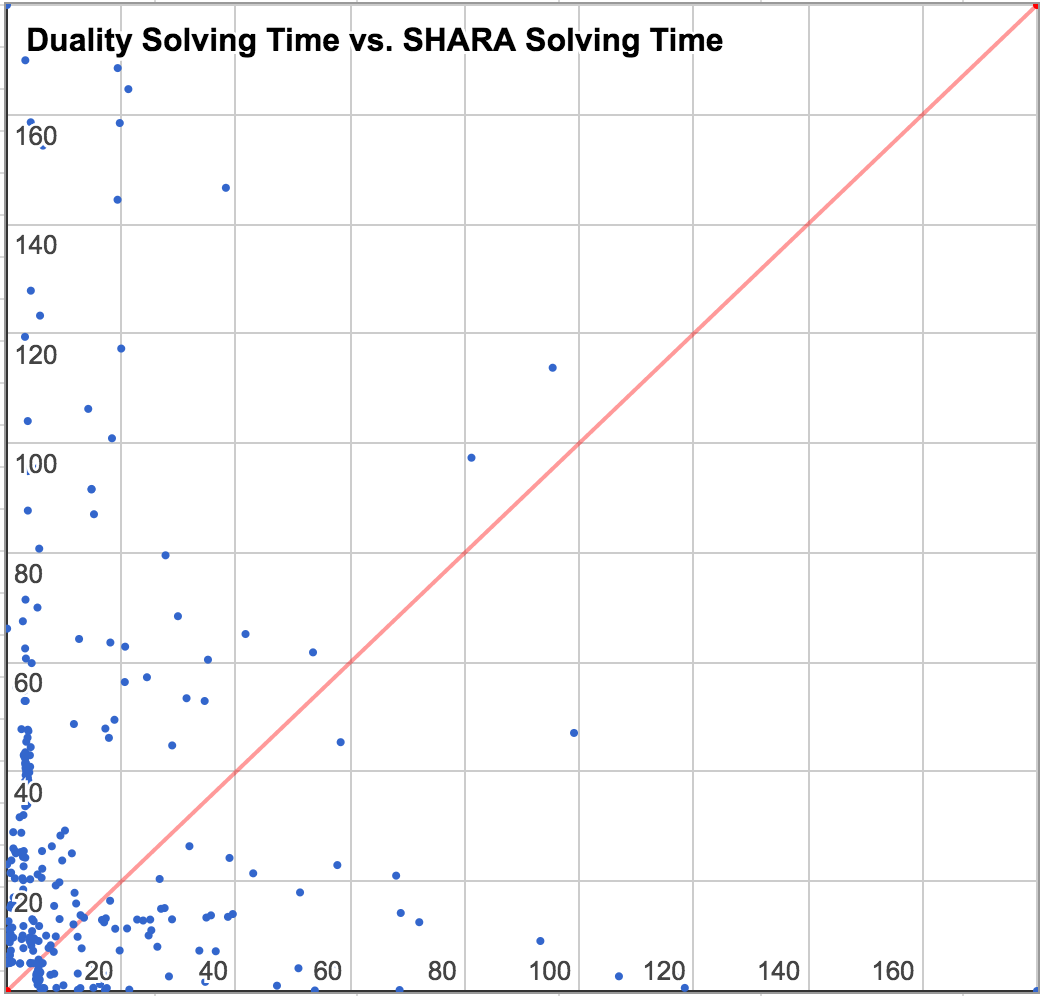
\includegraphics[width=\linewidth]{fig/complete.png} }
    %
    \ffigbox[.48\textwidth] %
    { \caption{Times of \sys and \duality vs. system size.
        %
        The $x$-axis ranges over the size of a given system, and the
        $y$-axis ranges over solvers' times.
        %
        Measurements of \sys and \duality are shown in blue and
        red, respectively. } %
      \label{fig:size} }
     { 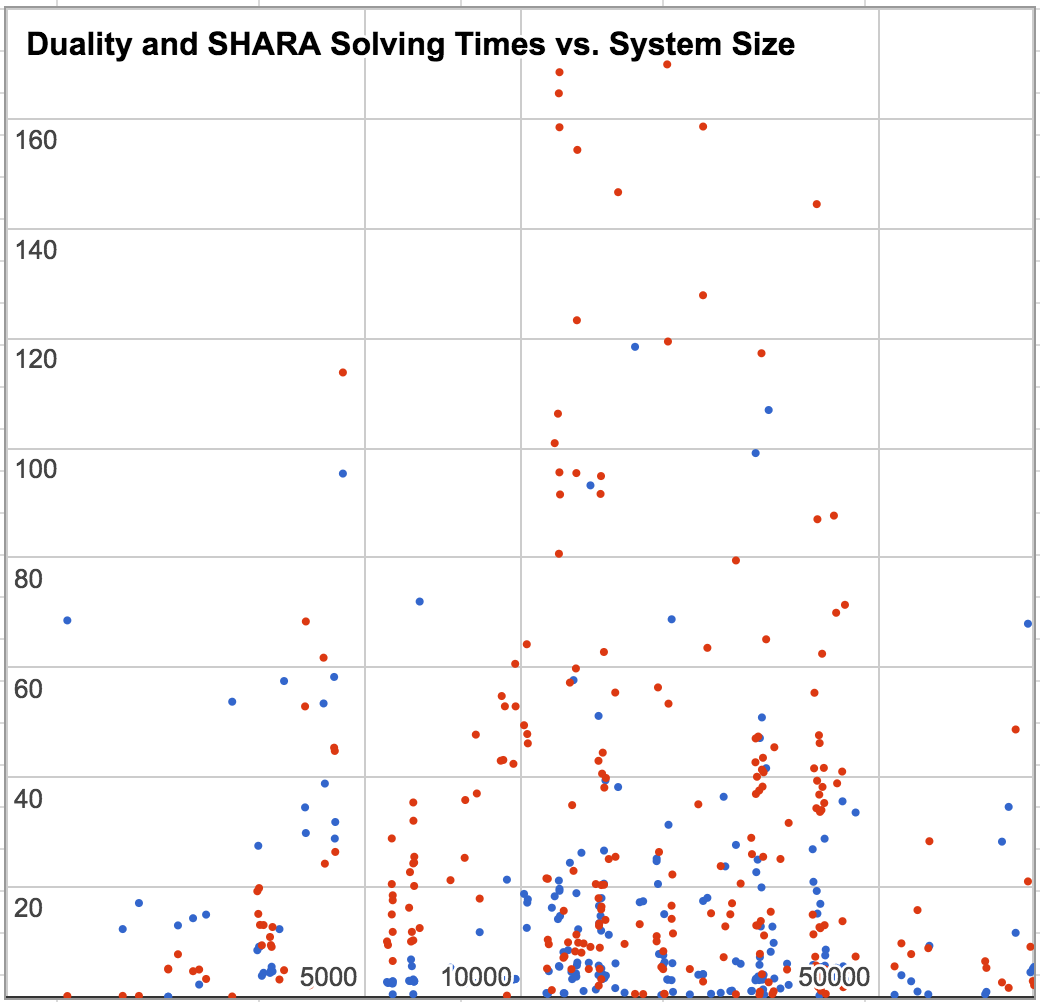
\includegraphics[width=\linewidth]{fig/size.png} }
  \end{floatrow}
\end{figure}
% introduce figure, summarize data not included:
The results of our evaluation are shown in
\autoref{fig:complete-data}.
%
Of the 4,040 benchmarks on which both solvers took a short amount
of time---less than five seconds---\sys solved the benchmarks in an
average of 0.51 seconds and \duality solved them in an average of 0.42
seconds.
%
\autoref{fig:complete-data} contains data for benchmarks which took
longer than five second for both systems to solve.
%
Out of these 269 benchmarks, \sys solved 185 in less time
than \duality, and solved 159 in less than half the time of \duality.
%
\duality solved 84 in less time than \sys, and solved 53 in less than
half the time of \sys.
%
Of the 762 benchmarks on which \sys timed out, \duality solved or
found a counterexample to 185.
%
Of the 1,145 benchmarks on which \duality timed out, \sys solved or
found a counterexample to 470.

% analyze data on system size:
\autoref{fig:size} shows the relationship between the solving times of
\duality and \sys and the size of a given system, measured as lines of
code in the format generated by \seahorn.
%
The majority of files have between 1,000 and 100,000 lines, so
\autoref{fig:size} is restricted to this range.
%
The data indicates that that performance improvement of \sys compared
to \duality is consistent across systems of all sizes available.

%result is good
The results indicate that \textbf{(1)} on a significant number of
different verification problems, \sys can perform significantly better than
\duality, but
%
\textbf{(2)} there are some cases in which the strengths of each
algorithm yield better results.
%
We collected the differences between sizes of a given system and its
minimal CDD expansion generated by \sys and found that they were
independent of \sys's performance compared to \duality.
%
Thus, while \duality may in the worst case enumerate exponentially
many derivation trees, it appears to enumerate far fewer
than the worst-case bound in some cases, causing it to perform better
than \sys.
%
Our results indicate that a third approach that combines the strengths
of both \duality and \sys, perhaps by lazily unwinding a given
recursion free system into a series of CDD systems instead of
derivation trees, could yield further improvements.

%%% Local Variables: 
%%% mode: latex
%%% TeX-master: "p"
%%% End: 


\section{Related Work}
\label{sec:related-work}
% different classes of CHC solvers:
A significant body of previous work has presented solvers for
different classes of Constrained Horn Clauses, or finding inductive
invariants of programs that correspond to solutions of CHCs.
% solving linear systems:
\impact attempts to verify a given sequential procedure, which
corresponds to solving a recursive linear CHC
system~\cite{mcmillan06}.
%
\impact attempts to verify a given procedure by iteratively selecting
paths and synthesizing invariants for each path.
%
Such an approach corresponds to iteratively and selecting and solving
derivations of a corresponding linear CHC system.

% interprocedural verification:
Previous work also proposed a verifier for recursive
programs~\cite{heizmann10}.
%
The proposed approach selects interprocedural paths of a program and
synthesizes invariants for each as nested interpolants.
%
Such an approach corresponds to attempting to solve a recursive CHC
system $S$ by selecting derivation trees of $S$
and solving each tree.

% solving recursive systems:
Previous work has proposed solvers for recursive systems that, given a
system $S$, attempt to solve $S$ by generating and
solving a series of recursion-free unwindings of $S$.

%
In particular, \eldarica attempts to solve each unwinding
$S'$ by reducing to and solving body-disjoint systems~\cite{rummer13a,rummer13b}.
%

%
\duality attempts to avoid solving all 
derivation-trees (i.e body-disjoint system) by using lazy annotation~\cite{bjorner13}.
%
Other optimizations selects derivation trees to solve using symbolic
symbolic analogs of Prolog evaluation with
tabling~\cite{jaffar09,mcmillan14}.
%

\whale attempts to verify a sequential recursive program by generating
and solving hierarchical programs (i.e., programs that may contain
conditional branches and procedure calls, but do not contain loops or
recursion), which correspond to recursion-free CHC
systems~\cite{albarghouthi12b}.
%
To solve a particular recursion-free system $S$, \whale
generates a linear inlining $S'$ of $S$ and solves
it using a procedure \vinta~\cite{albarghouthi12a}.
%
In general, $S'$ may have size exponential in the size of
$S$.

% compare sys to all of the previous work:
\sys is similar to all of the approaches given above for solving 
recursion-free CHC systems in that it reduces the problem of solving a
given recursion-free CHC system $S$ to solving a CHC system
in a directly-solvable class.
%


\sys is distinct from all of the approaches given above in that it
reduces solving a recursion-free CHC system to solving a
Clause-Dependent Disjoint (CDD) system.
%
CDD systems strictly contain the union of all classes of
directly-solvable CHC systems used by the above approaches, and can
themselves be solved directly.

%
For solving genreal CHC system, \sys uses the same strategy that proposed
by above approaches, that solving a series recursion-free CHC system that unwinding 
from the original CHC system, and try to synthesize the solution for the original 
CHC system by using solutions of recursion-free CHC systems.  

% bullshit CADE papers:
Previous work has given solvers for non-linear Horn clauses over
particular theories.
%
In particular, verifiers have been proposed for recursion-free systems
over the theory of linear arithmetic~\cite{komuravelli14}.
%
Because the verifier relies on quantifier elimination, it is not clear
if it can be extended to richer theories that support interpolation,
such as the combination of linear arithmetic with uninterpreted
functions.
%
Other work gives a solver for the class of \emph{timed pushdown
  systems}, a subclass of CHC systems over the theory of linear real
arithmetic~\cite{hoder12}.
%
Unlike both approaches, \sys can solve systems over any theory that
supports interpolation.

% DAG inlining:
DAG inlining, given a hierarchical program $P$, attempts to generate a
compact verification condition for $P$~\cite{lal-qadeer15}.
%
\sys contains a procedure that, given a recursion-free Horn Clause
system $S$, attempts to construct a compact CDD system
$S'$ such that each solution of $S'$ defines a
solution of $S$.
%
Because hierarchical programs and recursion-free Horn Clauses
correspond closely to each other, algorithms that operate on
hierarchical programs directly correspond to algorithms that operate
on recursion-free Horn Clauses.
%
However, an algorithm for constructing a verification condition of
hierarchical programs cannot apparently be directly used to synthesize
a solution of a recursion-free CHC system.

%%% Local Variables: 
%%% mode: latex
%%% TeX-master: "p"
%%% End: 


\section{Generating a Minimal CDD Expansion}
\label{app:cons-cdd}
% algorithm for constructing a CDD system:
\begin{algorithm}[t]
  % Declare IO markers.
  \SetKwInOut{Input}{Input}
  %
  \SetKwInOut{Output}{Output}
  % Declare sub-program (procedure) markers.
  \SetKwProg{myproc}{Procedure}{}{}
  % Inputs: a heap program and an error location.
  \Input{A recursion-free CHC system $S$.}
  % Output: inductive invariants.
  \Output{A minimal CDD expansion $S'$ of $S$ and
    a correspondence from $S'$ to $S$.} %
  \myproc{$\expand(S)$ %
    \label{line:expand-begin} }{ %
    % auxiliary procedure:
    \myproc{$\expandaux(S')$
      \label{line:expand-aux-begin} }{ %
      % case split: optional sharing clause:
      \Switch{$\sharingclause(S')$}{ %
        % case: no siblings with overlapping descendants
        \lCase{$\none$:}{ \Return{$S'$} %
          \label{line:expand-ret} } %
        % case: siblings with 
        \lCase{$C \in S', % 
          P \in \predof{S'}$: }{ %
          % expand the return:
          \Return{$\expandaux( %
            \copyrel(S', C, P))$ } %
          \label{line:expand-recurse}
        } %
      } %
    \label{line:expand-aux-end} } %
    % base call: 
    \Return{$( \expandaux(S), \corr )$ %
      \label{line:expand-base-call}}
  } %
  %
  \caption{$\expand$:
    given a recursion-free CHC system $S$, returns a minimal
    CDD expansion $S'$ of $S$ and its correspondence.}
  \label{alg:expand}
\end{algorithm}
%
% walk through top-level procedure:
Given a recursion-free CHC system $S$, \autoref{alg:expand} returns a
minimal CDD expansion of $S$ (\autoref{defn:min-expansion}).
%
$\expand$ defines a procedure $\expandaux$
(\autoref{line:expand-aux-begin}---\autoref{line:expand-aux-end}) that
takes a CHC system $S$ and returns a minimal CDD expansion of $S$.
%
$\expand$ runs $\expandaux$ on $S$ and
returns the result, paired with the map $\corr: \predof{S'} \to \predof{S}$ 
(\autoref{line:expand-base-call}).

% walk through aux procedure:
$\expandaux$, given a recursion-free CHC system $S'$,
runs a procedure $\sharingclause$ on $S'$, which tries to
find a clause $C \in S'$ and a predicate $P \in \bodyof{C}$
such that $P$ is in the transitive dependencies of two sibling
predicates.
%
In such a case, we say that $(C, P)$ is a
\emph{sibling-shared dependency}.

% case: no sibling-shares
If $\sharingclause$ determines that no sibling-shared dependency
exists, then $\expandaux$ returns $S'$
(\autoref{line:expand-ret}).

% case: there is a sibling-shared dependency:
Otherwise, $\sharingclause$ must have located a sibling-shared
dependency $(C, P)$. In this case, $\expandaux$ runs $\copyrel $ on
$S'$, $C$, and $P$, which returns an expansion of $S'$ by creating a
fresh copy of $P$ and updating $\bodyof{C}$ to avoid the shared
dependency.
%
$\expandaux$ recurses on this expansion and returns the result
(\autoref{line:expand-recurse}).
%

% CDD systems:
$\expand$ always returns a CDD expansion of its input
(see \autoref{app:corr}, \autoref{lem:expand-corr}) that is minimal.
% discussion: there are variations:
$\expand$ is certainly not unique as an algorithm for
generating a minimal CDD expansion.
%
In particular, feasible variations of $\expand$ can be
generated from different implementations of $\sharingclause$, each of
which chooses clause-relation pairs to return based on different
heuristics.
%
We expect that other expansion algorithms can also be developed by
generalizing algorithms introduced in previous work on generating
compact verification conditions of hierarchical
programs~\cite{lal-qadeer15}.

\section{Proof of characterization of CDD systems}
\label{app:char}
The following is a proof of \autoref{thm:cdd-contains}.
%
\begin{proof}
  % proof structure:
  To prove that CDD is a strict superset of the union of the class
  of linear systems and the class of body-disjoint systems, we prove
  %
  \textbf{(1)} CDD contains the class of linear systems,
  \textbf{(2)} CDD contains the class of body-disjoint systems, and
  \textbf{(3)} there is some CDD system that is neither linear nor
  body-disjoint.

  % contains linear systems:
  For goal \textbf{(1)}, let $S$ be an arbitrary linear
  system.
  %
  $S$ is CDD if for each clause $C$ in
  $S$ \textbf{(1)} and each pair of distinct predicates in
  the body of $C$ has disjoint transitive dependencies and
  \textbf{(2)} no predicate appears more than once in the body of $C$.
  (\autoref{defn:cdds}).
  %
  Let $C$ be an arbitrary clause in $S$.
  %
  Since $C$ is a linear clause, it has at most one relational
  predicate in its body. And since the system is recursion-free, the
  transitive dependencies are trivially disjoint and there can be no
  repeated predicate.
  %
  Therefore, $S$ is CDD.

  % contains body-disjoint systems:
  For goal \textbf{(2)}, let $S$ be an arbitrary
  body-disjoint system.
  %
  The dependence relation of $S$ is a tree $T$, by the
  definition of a body-disjoint system.
  %
  Let $C$ be an arbitrary clause in $S$, with
  distinct relational predicates $R_0$ and $R_1$ in its body.
  %
  All dependencies of $R_0$ and $R_1$ are in subtrees of $T$, which
  are disjoint by the definition of a tree.
  %
  Thus, $S$ is CDD, by \autoref{defn:cdds}.

  % distinguishing example:
  For goal \textbf{(3)}, the system $\mcchc$ is CDD, but is neither linear
  nor body-disjoint.
\end{proof}

\section{Proof $\solvecdd$ is in co-NP}
\label{app:solve-cp}
The following is a proof of \autoref{thm:solve-cp}.
%
Namely, $\solvecdd$ is in co-NP.
%
\begin{proof}
  $\prectr$ and $\postctr$ construct formulas linear in the size of the
  CHC system. The satisfiability problem for the constructed formulas
  are in NP for linear arithmetic.
  %
  $\solvecdd$ issues (at worst) a linear number of interpolation
  queries in terms of number of predicate.
  %
  Therefore, the upper bound of $\solvecdd$ is co-NP.
\end{proof}

\section{Proof of Correctness}
\label{app:corr}
%
In this section, we prove that \sys is correct when applied to
recursion-free CHC systems.
%
We first establish lemmas for the correctness of each procedure used
by \sys, namely \textsc{Collapse} (\autoref{lem:expansion-sound} and
\autoref{lem:expansion-complete}), $\expand$
(\autoref{lem:expand-corr}), and $\solvecdd$
(\autoref{lem:vc}, \autoref{lem:cdd-soln-sound}, and
\autoref{lem:cdd-soln-complete}).
%
We combine the lemmas to prove \sys is correct (\autoref{thm:corr}).

% lem: result connecting expansions to constructing solutions
For two recursion-free CHC systems $S$ and $S'$, if $S'$ is
an expansion of $S$, then the result of collapsing a
solution of $S'$ is a solution of $S$.
%
\begin{lem}
  \label{lem:expansion-sound}
  For two recursion-free CHC system $S'$ and $S$ such that $\sigma'$
  is a solution of $S'$ and $\eta$ is a correspondence from
  $S'$ to $S$, $\collapse{\eta}{\sigma'}$ is a
  solution of $S$.
\end{lem}
%
\begin{proof}
  % introduce 
  %
  For each predicate $P' \in \predof{S'}$ such that $\eta(P') = P$,
  there must exist some clause $C' \in S'$ such that $P' \in \bodyof{C'}$
  because $S'$ is an expansion of $S$.
  %
  Let predicate $Q' \in \predof{S'}$ be the head of $C'$.
  % 
  $\sigma'[P'] \land \consof{C'} \entails \sigma'[Q']$ by
  the fact that $\sigma'$ is a solution of $S'$.
  %
  Therefore,
  %
  \[ \collapse{ \eta }{ \sigma' }[P] \land \consof{C'} \entails %
  \left( \bigland_{ \substack{Q' \in \predof{S'} \\ \eta(Q') = Q} }
  \sigma(Q') = %
  \collapse{\eta}{\sigma'}[Q'] \right)
  \]
  % 
  Therefore, $\collapse{\eta}{\sigma'}$ has a solution for $P$.
  %
  Since $\collapse{\eta}{\sigma'}$ has a solution for each predicate
  in $S$, $\collapse{\eta}{\sigma'}$ is a solution of $S$.
\end{proof}

Every expansion of a solvable recursion-free CHC system is also
solvable.
% completeness of expansions:
\begin{lem}
  \label{lem:expansion-complete}
  If a recursion-free CHC system $S$ is solvable and
  $S'$ is an expansion of $S$, then $S'$ is solvable.
\end{lem}
%
\begin{proof}
  Let $\sigma$ be a solution of $S$, and let $\eta$ be a
  correspondence from $S'$ to $S$.
  %
  Let $\sigma'$ be such that for each $P' \in \predof{S'}$,
  $\sigma'(P') = \sigma(\eta(P'))$.
  %
  Then $\sigma'$ is a solution of $S'$.
\end{proof}

% CDD systems:
$\expand$ always returns a CDD expansion of its input.
%
\begin{lem}
  \label{lem:expand-corr}
  For two recursion-free CHC systems $S$ and $S'$ and a correspondence
  from $S'$ to $S$, $\eta$, such that $(S', \eta) = \expand(S)$,
  $S'$ is a CDD system and an expansion of $S$.
\end{lem}
%
\begin{proof}
  By induction over the evaluation of $\expand$ on
  an arbitrary recursion-free CHC system $S$.
  % inductive fact:
  The inductive fact is that for each evaluation step
  $\corr$ is a correspondence from argument
  $S'$ to $S$.
  % base case:
  In the base case, \expandaux is called initially on $S$,
  by \autoref{alg:expand}.
  %
  $\corr$ is a correspondence from $S$ to itself, by the definition of
  $\corr$
  (\autoref{app:cons-cdd}).

  % inductive case:
  In the inductive case,
  $\expandaux$ constructs an argument
  $\copyrel(S, C, P)$
  where $C$ is a clause and $P$ is a predicate in $S$.
  $\expandaux$ recusively invokes itself with this argument.
  %
  For each recursion-free CHC system $S'$ generated by $\copyrel(S, C, P)$,
  $\corr$ is a correspondence from $S'$ to
  $S$ by definition of $\copyrel$
  (\autoref{app:cons-cdd}).
  %
  By this fact and the inductive hypothesis, $\corr$ is
  a correspondence from $\copyrel(S',
  C, P)$ to $S$.

  % final claim: expand returns an expansion:
  $\expandaux$ returns its parameter at some step, by
  \autoref{alg:expand}.
  %
  Therefore, $\expandaux$ returns an expansion of $S$.

  % prove that returned system is CDD:
  For a given recursion-free CHC system $S'$, if $(S', \eta) =
  \expand(S')$,
  then $\sharingclause(S') = \none$, by the definition of $\expand$.
  %
  If $\sharingclause(S') = \none$, then $S'$ is
  CDD, by the definition of $\sharingclause$ and CDD systems
  (\autoref{defn:cdds}).
  %
  Therefore, $S'$ is CDD.
\end{proof}
%
Furthermore, $\expand$ returns a \emph{minimal} CDD
expansion of its input.
%
This fact is not required to prove \autoref{thm:corr}, and thus a
complete proof is withheld.

% lem: VC's characterize system sat:
For each recursion-free CHC system $S$, $S$ has a solution if and only
if all interpolation queries return interpolants.
%
\begin{lem}
  \label{lem:vc}
  Given a recursion-free CHC system $S$ that is CDD and solvable, for
  all predicates $P \in \predof{S}$,
  $\solveitp$ returns
  an interpolant $I$.
\end{lem}
%
\begin{proof}
  %
  Assume that $S$ has a solution $\sigma$ and there are some
  predicates $P \in \predof{S}$ such that
  $\solveitp$
  returns $SAT$. This means there must be a model $m$ for the
  conjunction of $\prectr(\cc{P},\sigma')$ and
  $\postctr(\cc{P},\sigma')$.
  %
  But $\postctr(\cc{P},\sigma) = \false$, by the definition of
  a solution of a CHC system.
  %
  Therefore, there can be no such model $m$.
  %
  Therefore,
  $\solveitp$ always
  returns interpolant.
\end{proof}

\begin{lem}
  \label{lem:solve-aux}
  Given a recursion-free CHC system $S$ that is CDD, if for all
  predicates $P \in \predof{S}$,
  $\solveitp$ returns
  an interpolant $I$, then $\solvecdd(S)$ is a solution of $S$.
\end{lem}
%
\begin{proof}
  % overview of structure:
  By induction on the $\solvecdd(S)$ calls to $\solveitp$ over all
  predicates $P \in \predof{S}$
  in topological order.
  %
  The inductive fact is that after each call to $\solveitp$, $\sigma$
  is a partial solution of $S$.
  % base case:
  In the base case, $\predof{S} = \varnothing$,
  %
  Therefore, $\sigma$ is a solution of $S$.

  % inductive case:
  In the inductive case, $\solvecdd$ calls $\solveitp$ on a predicate
  $P \in \predof{S}$ with partial solution $\sigma$.  Due to the
  topological ordering, $\sigma$ contains interpretations for each
  predicate $P \in \depsof{S}$.
  %
  Based on the definition of an interpolant (\autoref{defn:itps}),
  $\prectr(\cc{P},\sigma)$ and $\postctr(\cc{P},\sigma)$ are
  inconsistent.
  %
  The interpolant of these two formulas returned by $\solveitp$, $I$,
  is entailed by each clause $C$ where $P$ is the head where the
  predicates in $\bodyof{C}$ are substituted by their interpretations
  in $\sigma$.
  %
  $I$ is also inconsistent with all constraints that appear after $P$
  that support the query clause.
  %
  Therefore, when $\solvecdd$ updates $\sigma$ by binding $P$ to $I$
  the result is a partial solution of $S$.
\end{proof}

% SolveCDD: establish soundness
The output of $\solvecdd$ is correct for a given input CDD system.
%
\begin{lem}
  \label{lem:cdd-soln-sound}
  For a given CDD system $S$, and $\sigma = \solvecdd(S)$, %
  $\sigma$ is a solution of $S$.
\end{lem}
%
\begin{proof}
  %
  The fact that $\solvecdd(S)$ returns $\sigma$ implies that for each
  predicate $P \in \predof{S}$,
  $\solveitp$ returns
  a valid interpolant (\autoref{alg:solve-cdd}).
  %
  Therefore, \autoref{lem:solve-aux} implies that \solvecdd~returns a
  complete solution of $S$.
\end{proof}

% SolveCDD: establish completeness
\begin{lem}
  \label{lem:cdd-soln-complete}
  For a CDD system $S$ such that $S$ is
  solvable, %
  there is some $\sigma$ such that %
  $\sigma = \solvecdd(S)$.
\end{lem}
%
\begin{proof}
  % final claim:
  For all predicates $P \in \predof{S}$, $\solveitp$ returns a
  interpolant $I$, by
  \autoref{lem:vc} and the fact that $S$ is solvable.
  %
  Therefore, by \autoref{lem:solve-aux} and the fact that
  $S$ is solvable, $\solvecdd(S)$ returns a
  solution of $S$.
\end{proof}

% proof of main theorem:
The output of \sys is correct for a given input CDD system.
(\autoref{sec:approach}, \autoref{thm:corr}).
%
\begin{proof}
  Given two recursion-free CHC systems $S$ and $S'$ and a
  $\eta$ such that $(S', \eta) = \expand(S)$,
  $S'$ is minimal CDD expansion of $S$ and $\eta$ is a correspondence
  from $S'$ to $S$ (\autoref{lem:expand-corr}).
  %
  Assume that $S$ is solvable. Then so is $S'$, by
  \autoref{lem:expansion-complete}.
  %
  Therefore, there exists some $\sigma'$ such that $\sigma' =
  \solvecdd(S')$, by the definition of $\shara$.
  %
  $\sigma'$ is a solution of $S'$, by \autoref{lem:cdd-soln-sound}.
  %
  $\collapse{ \eta }{ \sigma' }$ is a solution of $S$, by
  \autoref{lem:expansion-sound}.
  %
  Therefore, $\shara$ returns a valid solution of $S$.
\end{proof}


% bibliography:
\bibliographystyle{abbrv}
\small

\bibliography{p}


\end{document}
